\documentclass[14pt]{extbook}
\usepackage{multicol, enumerate, enumitem, hyperref, color, soul, setspace, parskip, fancyhdr} %General Packages
\usepackage{amssymb, amsthm, amsmath, bbm, latexsym, units, mathtools} %Math Packages
\everymath{\displaystyle} %All math in Display Style
% Packages with additional options
\usepackage[headsep=0.5cm,headheight=12pt, left=1 in,right= 1 in,top= 1 in,bottom= 1 in]{geometry}
\usepackage[usenames,dvipsnames]{xcolor}
\usepackage{dashrule}  % Package to use the command below to create lines between items
\newcommand{\litem}[1]{\item#1\hspace*{-1cm}\rule{\textwidth}{0.4pt}}
\pagestyle{fancy}
\lhead{Progress Quiz 10}
\chead{}
\rhead{Version C}
\lfoot{6232-9639}
\cfoot{}
\rfoot{Fall 2020}
\begin{document}

\begin{enumerate}
\litem{
Determine the domain of the function below.\[ f(x) = \frac{4}{12x^{2} -32 x + 20} \]\begin{enumerate}[label=\Alph*.]
\item \( \text{All Real numbers except } x = a, \text{ where } a \in [0.72, 1.63] \)
\item \( \text{All Real numbers.} \)
\item \( \text{All Real numbers except } x = a \text{ and } x = b, \text{ where } a \in [14.99, 15.36] \text{ and } b \in [15.62, 16.64] \)
\item \( \text{All Real numbers except } x = a \text{ and } x = b, \text{ where } a \in [0.72, 1.63] \text{ and } b \in [1.55, 2.28] \)
\item \( \text{All Real numbers except } x = a, \text{ where } a \in [14.99, 15.36] \)

\end{enumerate} }
\litem{
Choose the equation of the function graphed below.
\begin{center}
    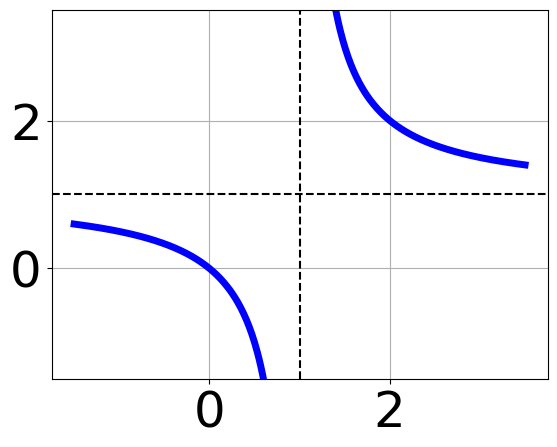
\includegraphics[width=0.5\textwidth]{../Figures/rationalGraphToEquationC.png}
\end{center}
\begin{enumerate}[label=\Alph*.]
\item \( f(x) = \frac{-1}{(x - 1)^2} + 1 \)
\item \( f(x) = \frac{1}{x + 1} + 1 \)
\item \( f(x) = \frac{1}{(x + 1)^2} + 1 \)
\item \( f(x) = \frac{-1}{x - 1} + 1 \)
\item \( \text{None of the above} \)

\end{enumerate} }
\litem{
Solve the rational equation below. Then, choose the interval(s) that the solution(s) belongs to.\[ \frac{-7x}{2x + 2} + \frac{-5x^{2}}{10x^{2} +24 x + 14} = \frac{-6}{5x + 7} \]\begin{enumerate}[label=\Alph*.]
\item \( x \in [-1.36,-0.99] \)
\item \( \text{All solutions lead to invalid or complex values in the equation.} \)
\item \( x_1 \in [0.2, 0.48] \text{ and } x_2 \in [-1.26,-1.09] \)
\item \( x_1 \in [0.2, 0.48] \text{ and } x_2 \in [-1.01,-0.99] \)
\item \( x \in [-1.56,-1.35] \)

\end{enumerate} }
\litem{
Solve the rational equation below. Then, choose the interval(s) that the solution(s) belongs to.\[ \frac{12}{-24x + 24} + 1 = \frac{12}{-24x + 24} \]\begin{enumerate}[label=\Alph*.]
\item \( x_1 \in [-2, 0] \text{ and } x_2 \in [-2,4] \)
\item \( \text{All solutions lead to invalid or complex values in the equation.} \)
\item \( x \in [1.0,2.0] \)
\item \( x_1 \in [1, 3] \text{ and } x_2 \in [-2,4] \)
\item \( x \in [-2,0] \)

\end{enumerate} }
\litem{
Choose the graph of the equation below.\[ f(x) = \frac{1}{(x + 3)^2} - 3 \]\begin{enumerate}[label=\Alph*.]
\begin{multicols}{2}\item 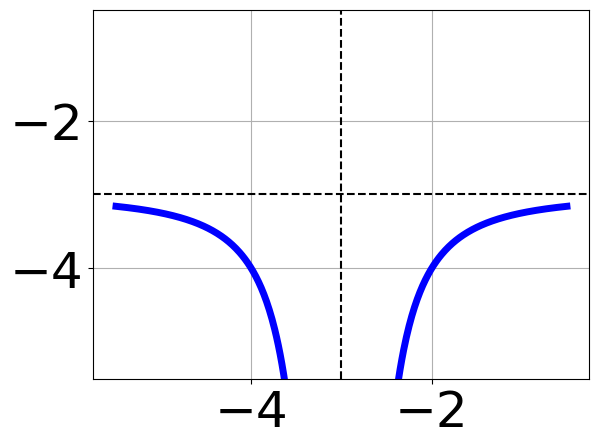
\includegraphics[width = 0.3\textwidth]{../Figures/rationalEquationToGraphAC.png}\item 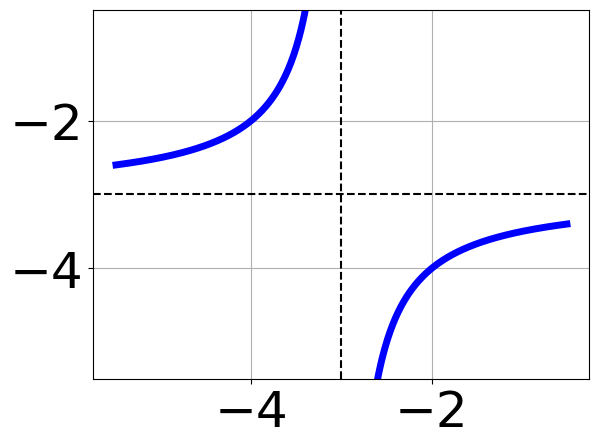
\includegraphics[width = 0.3\textwidth]{../Figures/rationalEquationToGraphBC.png}\item 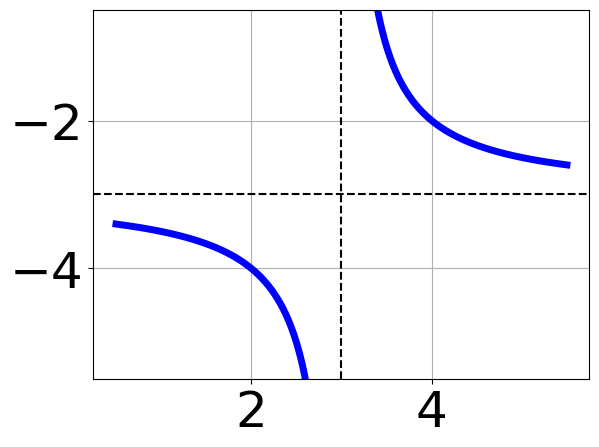
\includegraphics[width = 0.3\textwidth]{../Figures/rationalEquationToGraphCC.png}\item 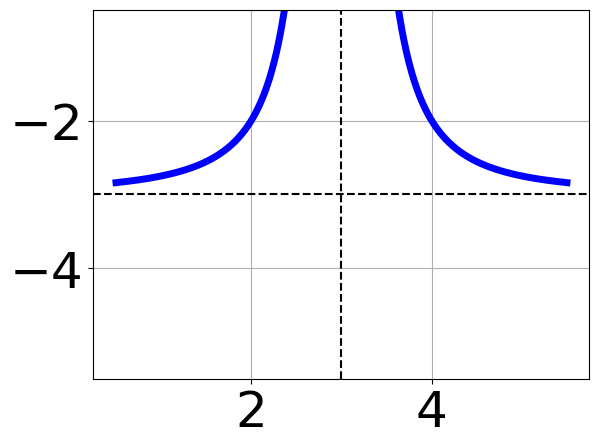
\includegraphics[width = 0.3\textwidth]{../Figures/rationalEquationToGraphDC.png}\end{multicols}\item None of the above.
\end{enumerate} }
\litem{
Solve the rational equation below. Then, choose the interval(s) that the solution(s) belongs to.\[ \frac{90}{40x + 60} + 1 = \frac{90}{40x + 60} \]\begin{enumerate}[label=\Alph*.]
\item \( x_1 \in [-3.5, 0.5] \text{ and } x_2 \in [-1.5,-0.5] \)
\item \( x \in [-1.5,-0.5] \)
\item \( x_1 \in [-3.5, 0.5] \text{ and } x_2 \in [1.5,3.5] \)
\item \( \text{All solutions lead to invalid or complex values in the equation.} \)
\item \( x \in [1.5,2.5] \)

\end{enumerate} }
\litem{
Determine the domain of the function below.\[ f(x) = \frac{4}{30x^{2} -43 x + 15} \]\begin{enumerate}[label=\Alph*.]
\item \( \text{All Real numbers except } x = a, \text{ where } a \in [14.82, 15.14] \)
\item \( \text{All Real numbers except } x = a \text{ and } x = b, \text{ where } a \in [14.82, 15.14] \text{ and } b \in [29.61, 30.49] \)
\item \( \text{All Real numbers.} \)
\item \( \text{All Real numbers except } x = a, \text{ where } a \in [0.57, 0.62] \)
\item \( \text{All Real numbers except } x = a \text{ and } x = b, \text{ where } a \in [0.57, 0.62] \text{ and } b \in [0.68, 1.16] \)

\end{enumerate} }
\litem{
Choose the graph of the equation below.\[ f(x) = \frac{-1}{x - 3} - 1 \]\begin{enumerate}[label=\Alph*.]
\begin{multicols}{2}\item 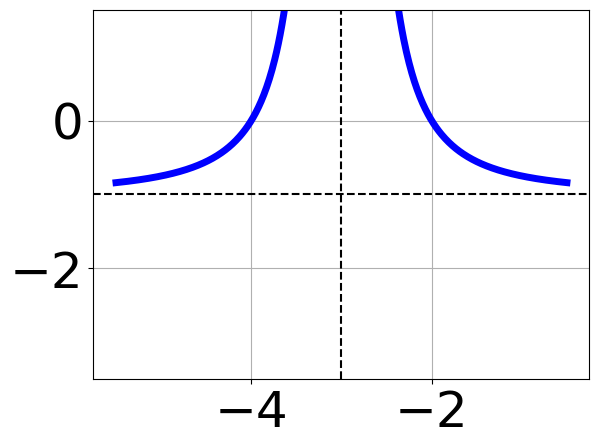
\includegraphics[width = 0.3\textwidth]{../Figures/rationalEquationToGraphCopyAC.png}\item 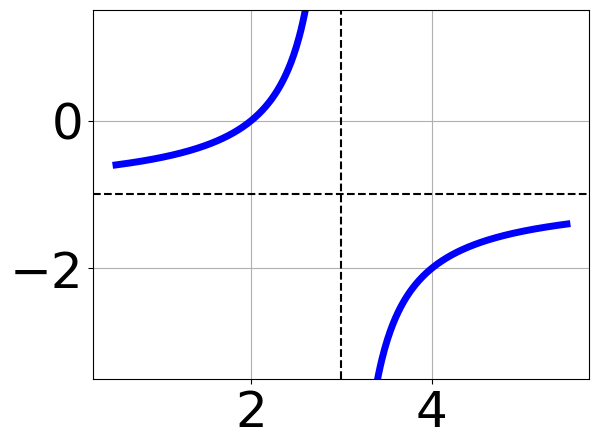
\includegraphics[width = 0.3\textwidth]{../Figures/rationalEquationToGraphCopyBC.png}\item 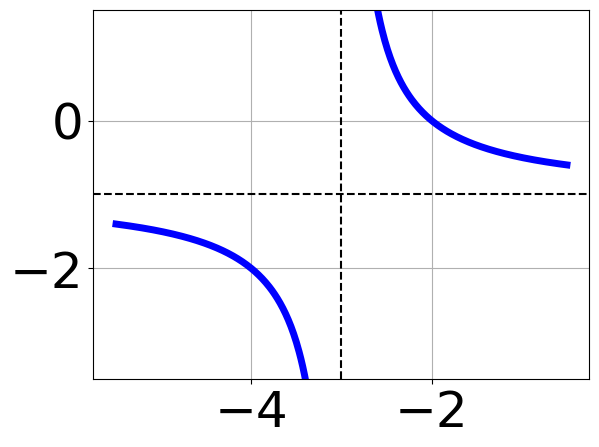
\includegraphics[width = 0.3\textwidth]{../Figures/rationalEquationToGraphCopyCC.png}\item 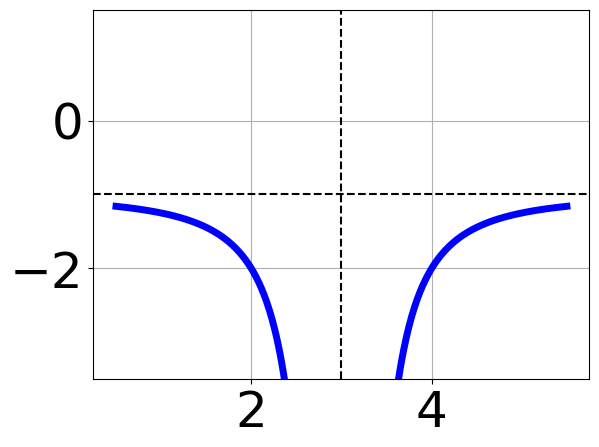
\includegraphics[width = 0.3\textwidth]{../Figures/rationalEquationToGraphCopyDC.png}\end{multicols}\item None of the above.
\end{enumerate} }
\litem{
Choose the equation of the function graphed below.
\begin{center}
    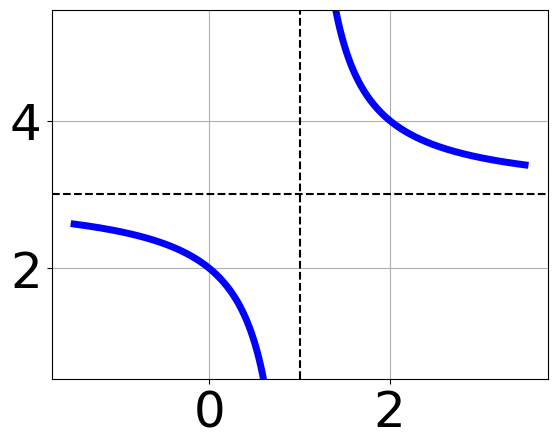
\includegraphics[width=0.5\textwidth]{../Figures/rationalGraphToEquationCopyC.png}
\end{center}
\begin{enumerate}[label=\Alph*.]
\item \( f(x) = \frac{-1}{(x - 1)^2} + 3 \)
\item \( f(x) = \frac{-1}{x - 1} + 3 \)
\item \( f(x) = \frac{1}{x + 1} + 3 \)
\item \( f(x) = \frac{1}{(x + 1)^2} + 3 \)
\item \( \text{None of the above} \)

\end{enumerate} }
\litem{
Solve the rational equation below. Then, choose the interval(s) that the solution(s) belongs to.\[ \frac{5x}{-2x + 7} + \frac{-7x^{2}}{8x^{2} -16 x -42} = \frac{-5}{-4x -6} \]\begin{enumerate}[label=\Alph*.]
\item \( x_1 \in [-0.08, 1.51] \text{ and } x_2 \in [3.5,5.5] \)
\item \( x \in [-3.4,-1.97] \)
\item \( x_1 \in [-0.08, 1.51] \text{ and } x_2 \in [-8.1,2.9] \)
\item \( \text{All solutions lead to invalid or complex values in the equation.} \)
\item \( x \in [-1.96,-0.9] \)

\end{enumerate} }
\end{enumerate}

\end{document}